\section{Results \& Discussion}

The pytokio implementation of TOKIO provides connectors for the following tools either available as community supported open-source tools or pre-installed on Cray systems:

\begin{itemize}
\item \textbf{Cray SDB} for node topology
\item \textbf{Slurm} to enable indexing based on job ID and node lists
\item \textbf{Darshan} for application-level I/O profiling
\item \textbf{Lustre} \texttt{lfs} and \texttt{lctl} for file system health
\item \textbf{LMT} to connect to the Sonexion Lustre monitoring tool service
\end{itemize}

Using these connectors to standard component-level tools, Unified Monitoring and Metrics Interfaces (UMAMI)~\cite{Lockwood2017} diagrams can be generated to present application performance alongside various dimensions of system health and contention over a computing campaign.  An example of an UMAMI diagram, shown in Figure \ref{fig:umami}, demonstrates a case where HACC write performance was abnormally low for a specific job during a time when LMT recorded significant bandwidth contention, OSS CPU load, and metadata contention.  As will be detailed in this work, aligning application performance data from Darshan with Lustre server-side data from LMT allows TOKIO to demonstrate how different I/O subsystem components contribute to performance loss in any job of interest.
% * <pcarns@gmail.com> 2018-01-19T16:21:36.773Z:
% 
% It seems like there should be some lead in text before the "Using these connectors" sentence to tie this text back to the four logical layers described earlier.  UMAMI and the heatmap thing are examples of "analysis applications" in that taxonomy, right?
% 
% ^.

\begin{figure}[t]
    \centering
    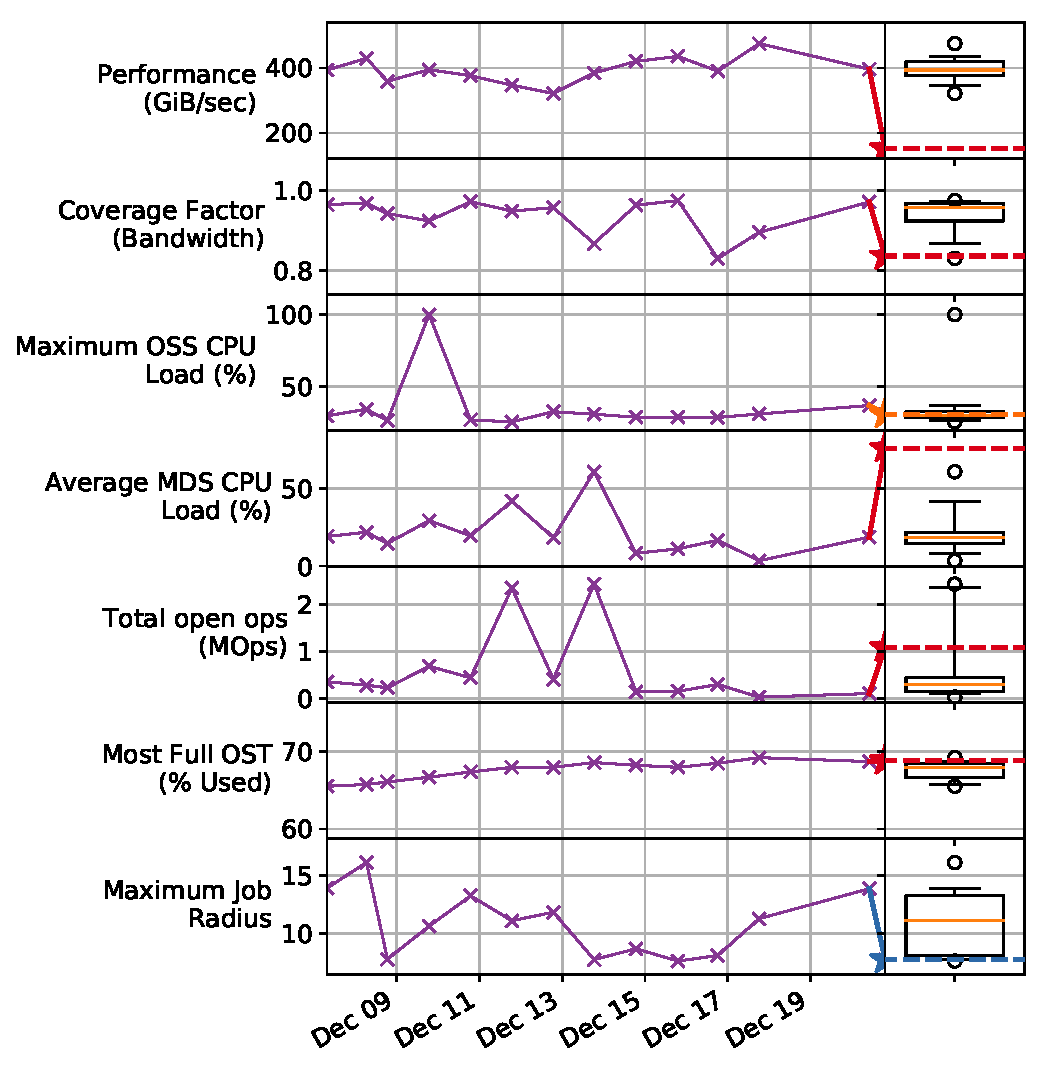
\includegraphics[width=1.0\columnwidth]{umami}
    \vspace{-.3in}
    \caption{Write rate of a stage-out operation from DataWarp to Lustre on Cori.  Each horizontal line represents a single OST performing intense I/O; better overall performance was obtained by manually pre-striping the DataWarp stage-out destination directory to ensure that the performance of all OSTs was available.}
    \label{fig:umami}
    \vspace{-.2in}
\end{figure}

In addition to analyzing performance variation across science campaigns, TOKIO provides a suite of tools to visualize systematic performance problems.  For example, a simple TOKIO LMT visualizer produced Figure \ref{fig:lustre-heatmap} and revealed that poor stage-out performance from DataWarp to Lustre, which occurs entirely outside the scope of user jobs and applications, resulted from poor striping.  Similarly, another TOKIO analysis examines Darshan logs \emph{en masse} to statistically correlate poor I/O performance with specific Lustre OSTs using the per-file performance and striping information encoded by the Darshan Lustre module~\cite{Snyder2016modular} to reveal potentially unhealthy OSTs.  Both of these tools will be presented in detail to demonstrate how meaningful analysis can be expressed in only several dozen lines of code using the pytokio package.

\begin{figure}[t]
    \centering
    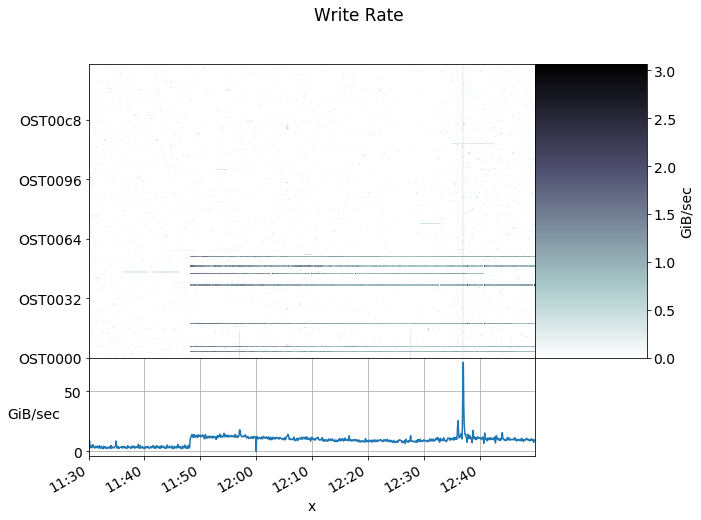
\includegraphics[width=1.0\columnwidth]{lustre-stageout-performance}
    \vspace{-.3in}
    \caption{Unified Monitoring and Metrics Interface (UMAMI) of a synthetic computational campaign of HACC~\cite{Habib2012} job runs performed on NERSC's Cori system over a week.  "Coverage Factor (BW)" is the fraction of global file system traffic originating from the HACC job, "Maximum Job Radius" represents the overall spread of each HACC job's allocated nodes across the dragonfly network, and the remaining metrics represent server-side Lustre data captured by LMT.}
    \label{fig:lustre-heatmap}
    \vspace{-.2in}
\end{figure}

The pytokio implementation is designed to use whatever tools are already available on any existing Cray XC and ClusterStor platform, and to demonstrate this, results from applying TOKIO on both the Cori system at NERSC and the Theta system at ALCF will be presented.  Furthermore, because pytokio is BSD-licensed and available freely on GitHub, new connectors to site-specific telemetry or future monitoring tools can be contributed to suit the needs of different sites' existing monitoring infrastructures.

% https://jupyter.nersc.gov/user/glock/notebooks/global/homes/g/glock/src/git/tokio-abcutils/sc18_reanalysis.ipynb

% \subsection{Subsection Heading Here}
% Subsection text here.

% \subsubsection{Subsubsection Heading Here}
% Subsubsection text here.
